\documentclass[a4paper, 10pt, fleqn]{article}

\usepackage[utf8]{inputenc}
\usepackage[T1]{fontenc}
\usepackage{textcomp}
\usepackage{lmodern}
\usepackage[ngerman]{babel}
\usepackage{tocbibind}
\usepackage{enumerate}
\usepackage{xcolor}
\usepackage{pdfpages}
\usepackage{amsmath}
\usepackage{graphicx}
\usepackage{geometry}
\usepackage{scrpage2}
\usepackage{lastpage}
\usepackage[hyphens]{url}
\usepackage{hyperref}
\usepackage{listings}
\usepackage{float}
\restylefloat{figure}
\lstset{language=[ansi]C++}

\newcommand{\code}[1]{\texttt{#1}}

\renewcommand*{\listoffigures}{%
  \begingroup
  \tocchapter
  \tocfile{\listfigurename}{lof}
  \endgroup
}

\geometry{left=3cm, top=3cm, bottom=3cm, right=2cm}

\hypersetup{
    colorlinks,
    linkcolor=black,
    citecolor=black,
    urlcolor=black
}

\pagestyle{scrheadings}
\ihead{APPE Team 13}\ohead{Systemspezifikation} 
\ifoot{\today} \ofoot{Seite \thepage\ von {\hypersetup{linkcolor=black}\pageref{LastPage}}}

% Einrücken zu Beginn von neuem Absatz unterdrücken
\setlength{\parindent}{0pt}

% Zeilenabstand einstellen
\usepackage{setspace}
\makeatletter
\newcommand{\MSonehalfspacing}{%
  \setstretch{1.44}%  default
  \ifcase \@ptsize \relax % 10pt
    \setstretch {1.448}%
  \or % 11pt
    \setstretch {1.399}%
  \or % 12pt
    \setstretch {1.433}%
  \fi
}
\newcommand{\MSdoublespacing}{%
  \setstretch {1.92}%  default
  \ifcase \@ptsize \relax % 10pt
    \setstretch {1.936}%
  \or % 11pt
    \setstretch {1.866}%
  \or % 12pt
    \setstretch {1.902}%
  \fi
}
\makeatother
\MSonehalfspacing


\begin{document}
% !TEX root = Dokumentation.tex
\begin{titlepage}   

\begin{center}
\textsc{\Large Team 13}\\[0.5cm]

% Title
\newcommand{\HRule}{\rule{\linewidth}{0.5mm}}
\HRule \\[0.4cm]
{ \huge \bfseries Filialbestellsystem}\\[0.4cm]
{ \LARGE \bfseries Projektmanagementplan}\\[0.4cm]
\HRule \\[1.5cm]

% Unterer Teil der Seite
{\large Rotkreuz, \today}

\begin{figure}[H]%Position festigen
\centering
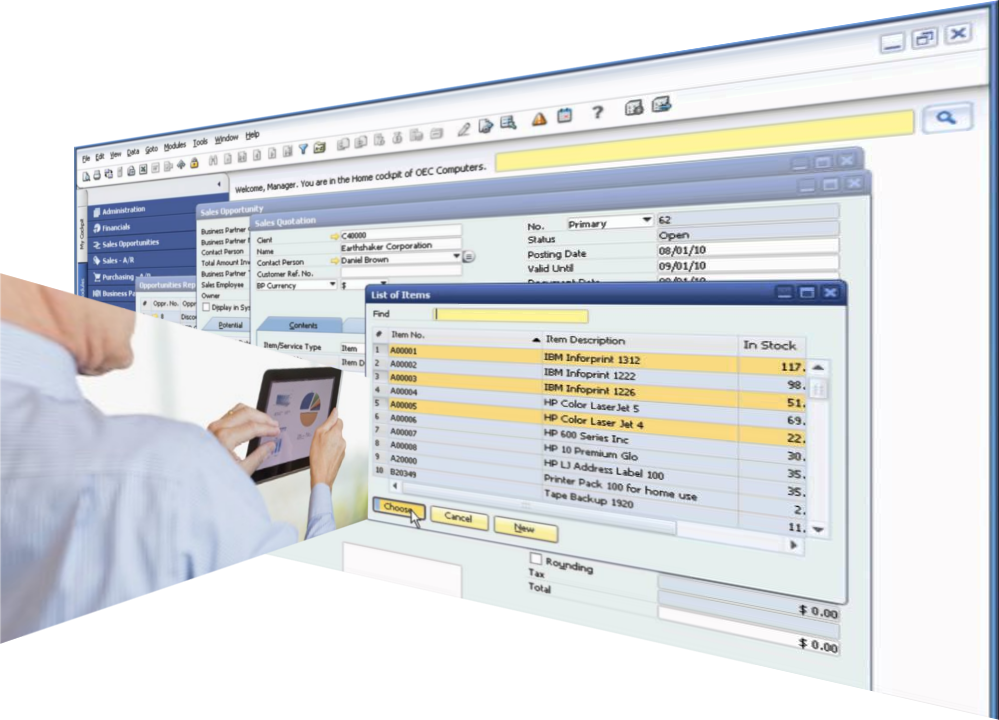
\includegraphics[width=0.7\textwidth]{Images/Titelbild.png}
\label{fig:title}
\end{figure}
% Author and supervisor
\begin{minipage}{0.4\textwidth}
\begin{flushleft} \large
\emph{Autoren:}\\
Marco Moro\\
Severin Gmür\\
Ramon Wyss\\
Tobias Kreienbühl\\
\end{flushleft}
\end{minipage}
\hfill
\begin{minipage}{0.4\textwidth}
\begin{flushright} \large
%\emph{Supervisor:} \\
%tbd
\end{flushright}
\end{minipage}
\large
\vfill
I.BA\_APPE.F1701 \\
Hochschule Luzern Informatik

\end{center}

\end{titlepage}
\tableofcontents
\clearpage
\section{Systemübersicht}

\section{Architektur und Designentscheide}
\subsection{Modell(e) und Sichten}
\subsubsection{Kontextdiagramm}

\subsubsection{UML-Klassendiagramme}

\subsubsection{Sequenzdiagramme}

\subsection{Entwurfsentscheide}

\section{Schnittstellen}
\subsection{Externe Schnittstellen}

\subsection{Wichtige Interne Schnittstellen}

\section{Environment-Anforderungen}

\end{document}